\documentclass[letterpaper,10pt]{article}
\usepackage[top=2cm, bottom=1.5cm, left=1cm, right=1cm]{geometry}
\usepackage{amsmath, amssymb, amsthm,graphicx}
\usepackage{fancyhdr}
\pagestyle{fancy}

\lhead{\today}
\chead{QE Assignment 10}
\rhead{Justin Hood}

\newcommand{\Z}{\mathbb{Z}}
\newcommand{\Q}{\mathbb{Q}}
\newcommand{\R}{\mathbb{R}}
\newcommand{\C}{\mathbb{C}}
\newtheorem{lem}{Lemma}

\begin{document}
\begin{enumerate}
\item We consider the tax error data. Given that we have only the $n$ and $np$ data, we will make a fraction nonconforming chart. We compute the LCL and UCL from the formulas in the text, noting that because the computed LCL is less than zero, we will round to zero for our analysis.
\begin{center}
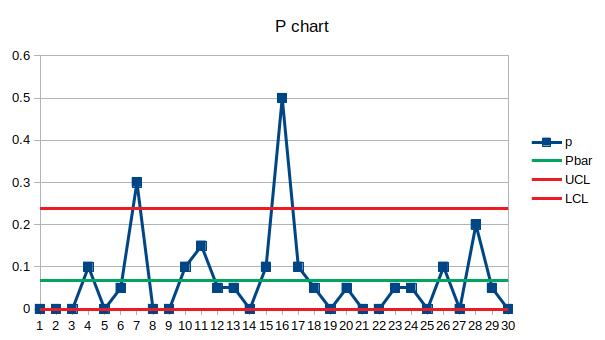
\includegraphics[scale=1]{1pchart.png}
\end{center}
We see that there are two data points that are above our computed upper limit. Aside from these, there does not appear to be any runs or trends that need to be investigated. As such, we will look at these two instances. If there is an assignable cause to why the number of nonconforming in these cases was high, such as a new accountant, or an improper form being used, we can remove these points, and reconduct the analysis. Otherwise, we see that this process is not within control.
\item We now consider the Traffic Fatality data. To begin, we construct a varaible $n$ control chart using the average number of samples to compute the UCL and LCL.
\begin{center}
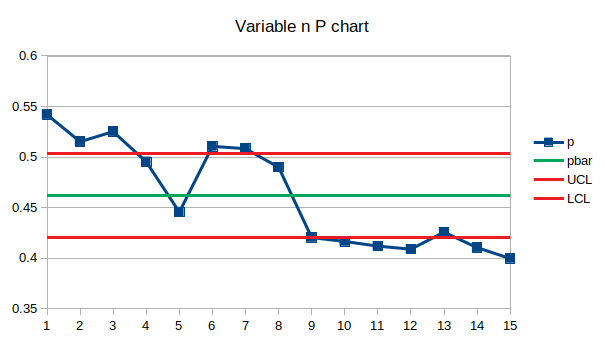
\includegraphics[scale=1]{2a.png}
\end{center}
We know that the data is for 15 consecutive years. At some point over the course of this timeline, in 1991, the county began an agressive anti DUI campaign. Looking at the $P$ chart, we see that the time can be split into two rough categories, with one corresponding to the presumed pre-campaign, and one post-campaign. We see that the earlier years have a significantly higher nonconforming percentage than the later years. Based on this, we see that the campaign appears to be effective, and the data should be reanalyzed using only the post-campaign for more accurate longer term control limits.
\item Finally, we consider the data in the ``case 2" file. We compute the $\bar{x}$ and $R$ control charts,
\begin{center}
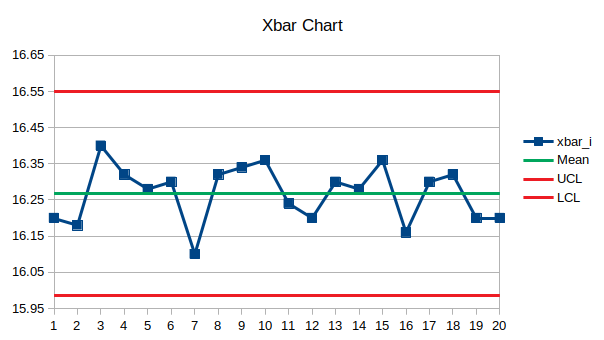
\includegraphics[scale=1]{3a.png}
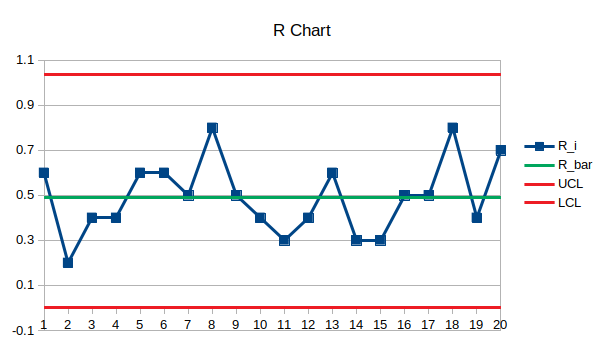
\includegraphics[scale=1]{3b.png}
\end{center}
And see that the process is within control. We then consider that the data is roughly normal from the following histogram,
\begin{center}
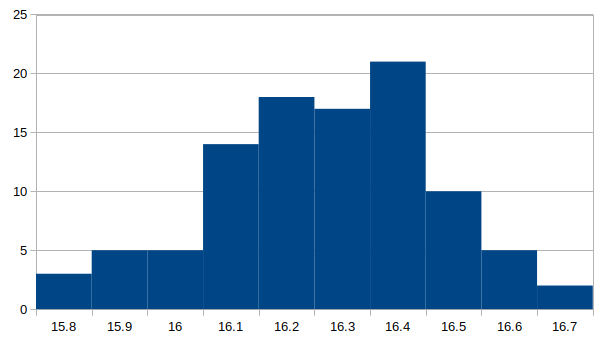
\includegraphics[scale=1]{3c.png}
\end{center}
As such, we compute,
\[\sigma_x=\frac{\bar{R}}{d_2}=\frac{0.49}{2.326}=0.210662\]
Assuming the limits defined as $16.2\pm 0.5$, we then consider the following shift of the center to be $\mu=16.5$. We then compute,
\[p(x>UCL)=p(x>16.7)=1-p(x\leq 16.7)=1-\Phi\left(\frac{16.7-16.5}{0.210662}\right)=1-\Phi(0.949388)=1-0.82879=0.17121\]
Thus, we see that the probability of the next sample being over the UCL is, roughly $17.12\%$.
\end{enumerate}
\end{document}
